\documentclass{ctexart}
\usepackage{geometry}
\usepackage{fancyhdr}
\usepackage{graphicx}
\usepackage{wrapfig}
\usepackage{booktabs}
\usepackage{amsmath}
\usepackage{tikz}
\usepackage{array}
\xeCJKsetup{CJKmath=true} 
\usepackage{zhnumber} % change section number to chinese
\renewcommand\thesection{\zhnum{section}}
\renewcommand \thesubsection {\arabic{subsection}}
\CTEXsetup[format={\Large\bfseries}]{section}

\geometry{
    a4paper,
    left=3.18cm,
    right=3.18cm,
    top=3.04cm,
    bottom=3.04cm
}

\pagestyle{fancy}
\fancyhf{}
\renewcommand{\headrulewidth}{0.7pt} % 设置页眉横线粗细
\fancyhead[L]{\kaishu\large 大学物理实验报告} % 在左侧设置页眉文字
\fancyhead[R]{\kaishu\large 哈尔滨工业大学(深圳) } % 在右侧设置页眉文字
\fancyfoot[R]{\thepage} % 将页数放在右下角


\setlength\headwidth{\textwidth}

\begin{document}

\noindent
\begin{center}
\textbf{
\begin{tabular}{p{2.4cm}p{2.4cm}p{4cm}p{4cm}}
    班级 \hrulefill & 学号 \hrulefill & 姓名 \hrulefill & 教师签字 \hrulefill \\
\end{tabular}
\begin{tabular}{p{6cm}p{3.6cm}p{3.6cm}}
    实验日期 \hrulefill & 预习成绩 \hrulefill & 总成绩 \hrulefill
\end{tabular}
{\noindent}	 \rule[-10pt]{\textwidth}{0.7pt}
}\end{center}

\begin{center}
    \Large \textbf{实验内容 \underline{迈克尔逊干涉仪}}
\end{center}

\section{预习}
\subsection{结合下图迈克尔逊干涉仪的等效光路图,推导出光程差的表达式$\Delta L = 2h \cos \alpha$。}
\begin{wrapfigure}{r}{0.5\textwidth}
    \centering
    \vspace{-0.8cm}
    \setlength{\belowcaptionskip}{-1cm}
    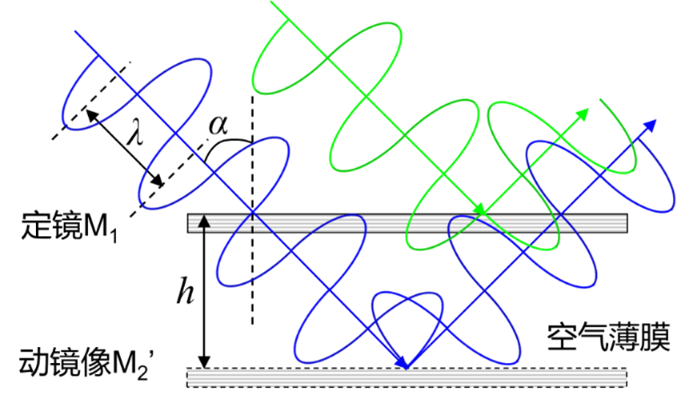
\includegraphics[width=0.45\textwidth]{./pic/mkex.png}
\end{wrapfigure}

~\\
~\\
~\\
~\\
~\\
~\\

\subsection{本实验将测量He-Ne激光的波长λ,若等倾干涉圆环每变化50环,动镜M2对应的螺旋测微器读数变化为d(注意:M2实际移动距离为d/20),根据光程差的表达式光程差ΔL = 2hcosα,结合中心圆环对应的倾角α ≈ 0这一近似条件,推导出波长λ的表达式(提示:光程差每改变1个波长,干涉圆环变化1环)。}

~\\
~\\
~\\
~\\
~\\
~\\

\section{实验目的及任务}
\subsection{了解迈克尔孙干涉仪的结构、原理及调节方法;}
\subsection{观察光的非定域和定域干涉现象,包括等倾和等厚干涉;}
\subsection{逐差法测定He-Ne激光波长;}
\subsection{作图法计算空气的折射率。}


\newpage
\section{原始数据记录}
\subsection{}
\begin{table}[!htbp]
    \renewcommand{\arraystretch}{1.2} % 表格行高倍数
    \centering
    \caption{测定$He-Ne$激光波长数据}
    \label{tab:HeNe}
    \begin{tabular}{|c|m{1.2cm}<{\centering}|m{1.2cm}<{\centering}|m{1.2cm}<{\centering}|m{1.2cm}<{\centering}|m{1.2cm}<{\centering}|m{1.2cm}<{\centering}|}
    \hline
    圆环变化数目 & 0 & 50 & 100 & 150 & 200 & 250 \\
    \hline
    $M_2$位置读数(mm) & & & & & &  \\
    \hline
    \end{tabular}
\end{table}

\subsection{}

\begin{table}[!htbp]
    \renewcommand{\arraystretch}{1.2} % 表格行高倍数
    \centering
    \caption{测定空气折射率数据}
    \label{tab:ref}
    \begin{tabular}{|c|m{2.4cm}<{\centering}|m{1.2cm}<{\centering}|m{1.2cm}<{\centering}|m{1.2cm}<{\centering}|m{1.2cm}<{\centering}|m{1.2cm}<{\centering}|}
    \hline
    测量次数 & $\Delta P (mm \ Hg)$ & 50 & 100 & 150 & 200 & 250 \\
    \hline
    1 & N & & & & &  \\
    \hline
    2 & N & & & & &  \\
    \hline
    3 & N & & & & &  \\
    \hline
    \multicolumn{2}{|c|}{$N$平均值} & & & & &  \\
    \hline
    \end{tabular}
\end{table}

\subsection{观察等倾和等厚现象,并附现象图。}

\begin{figure}[htbp]
    \begin{minipage}[t]{0.5\linewidth}
    \centering
    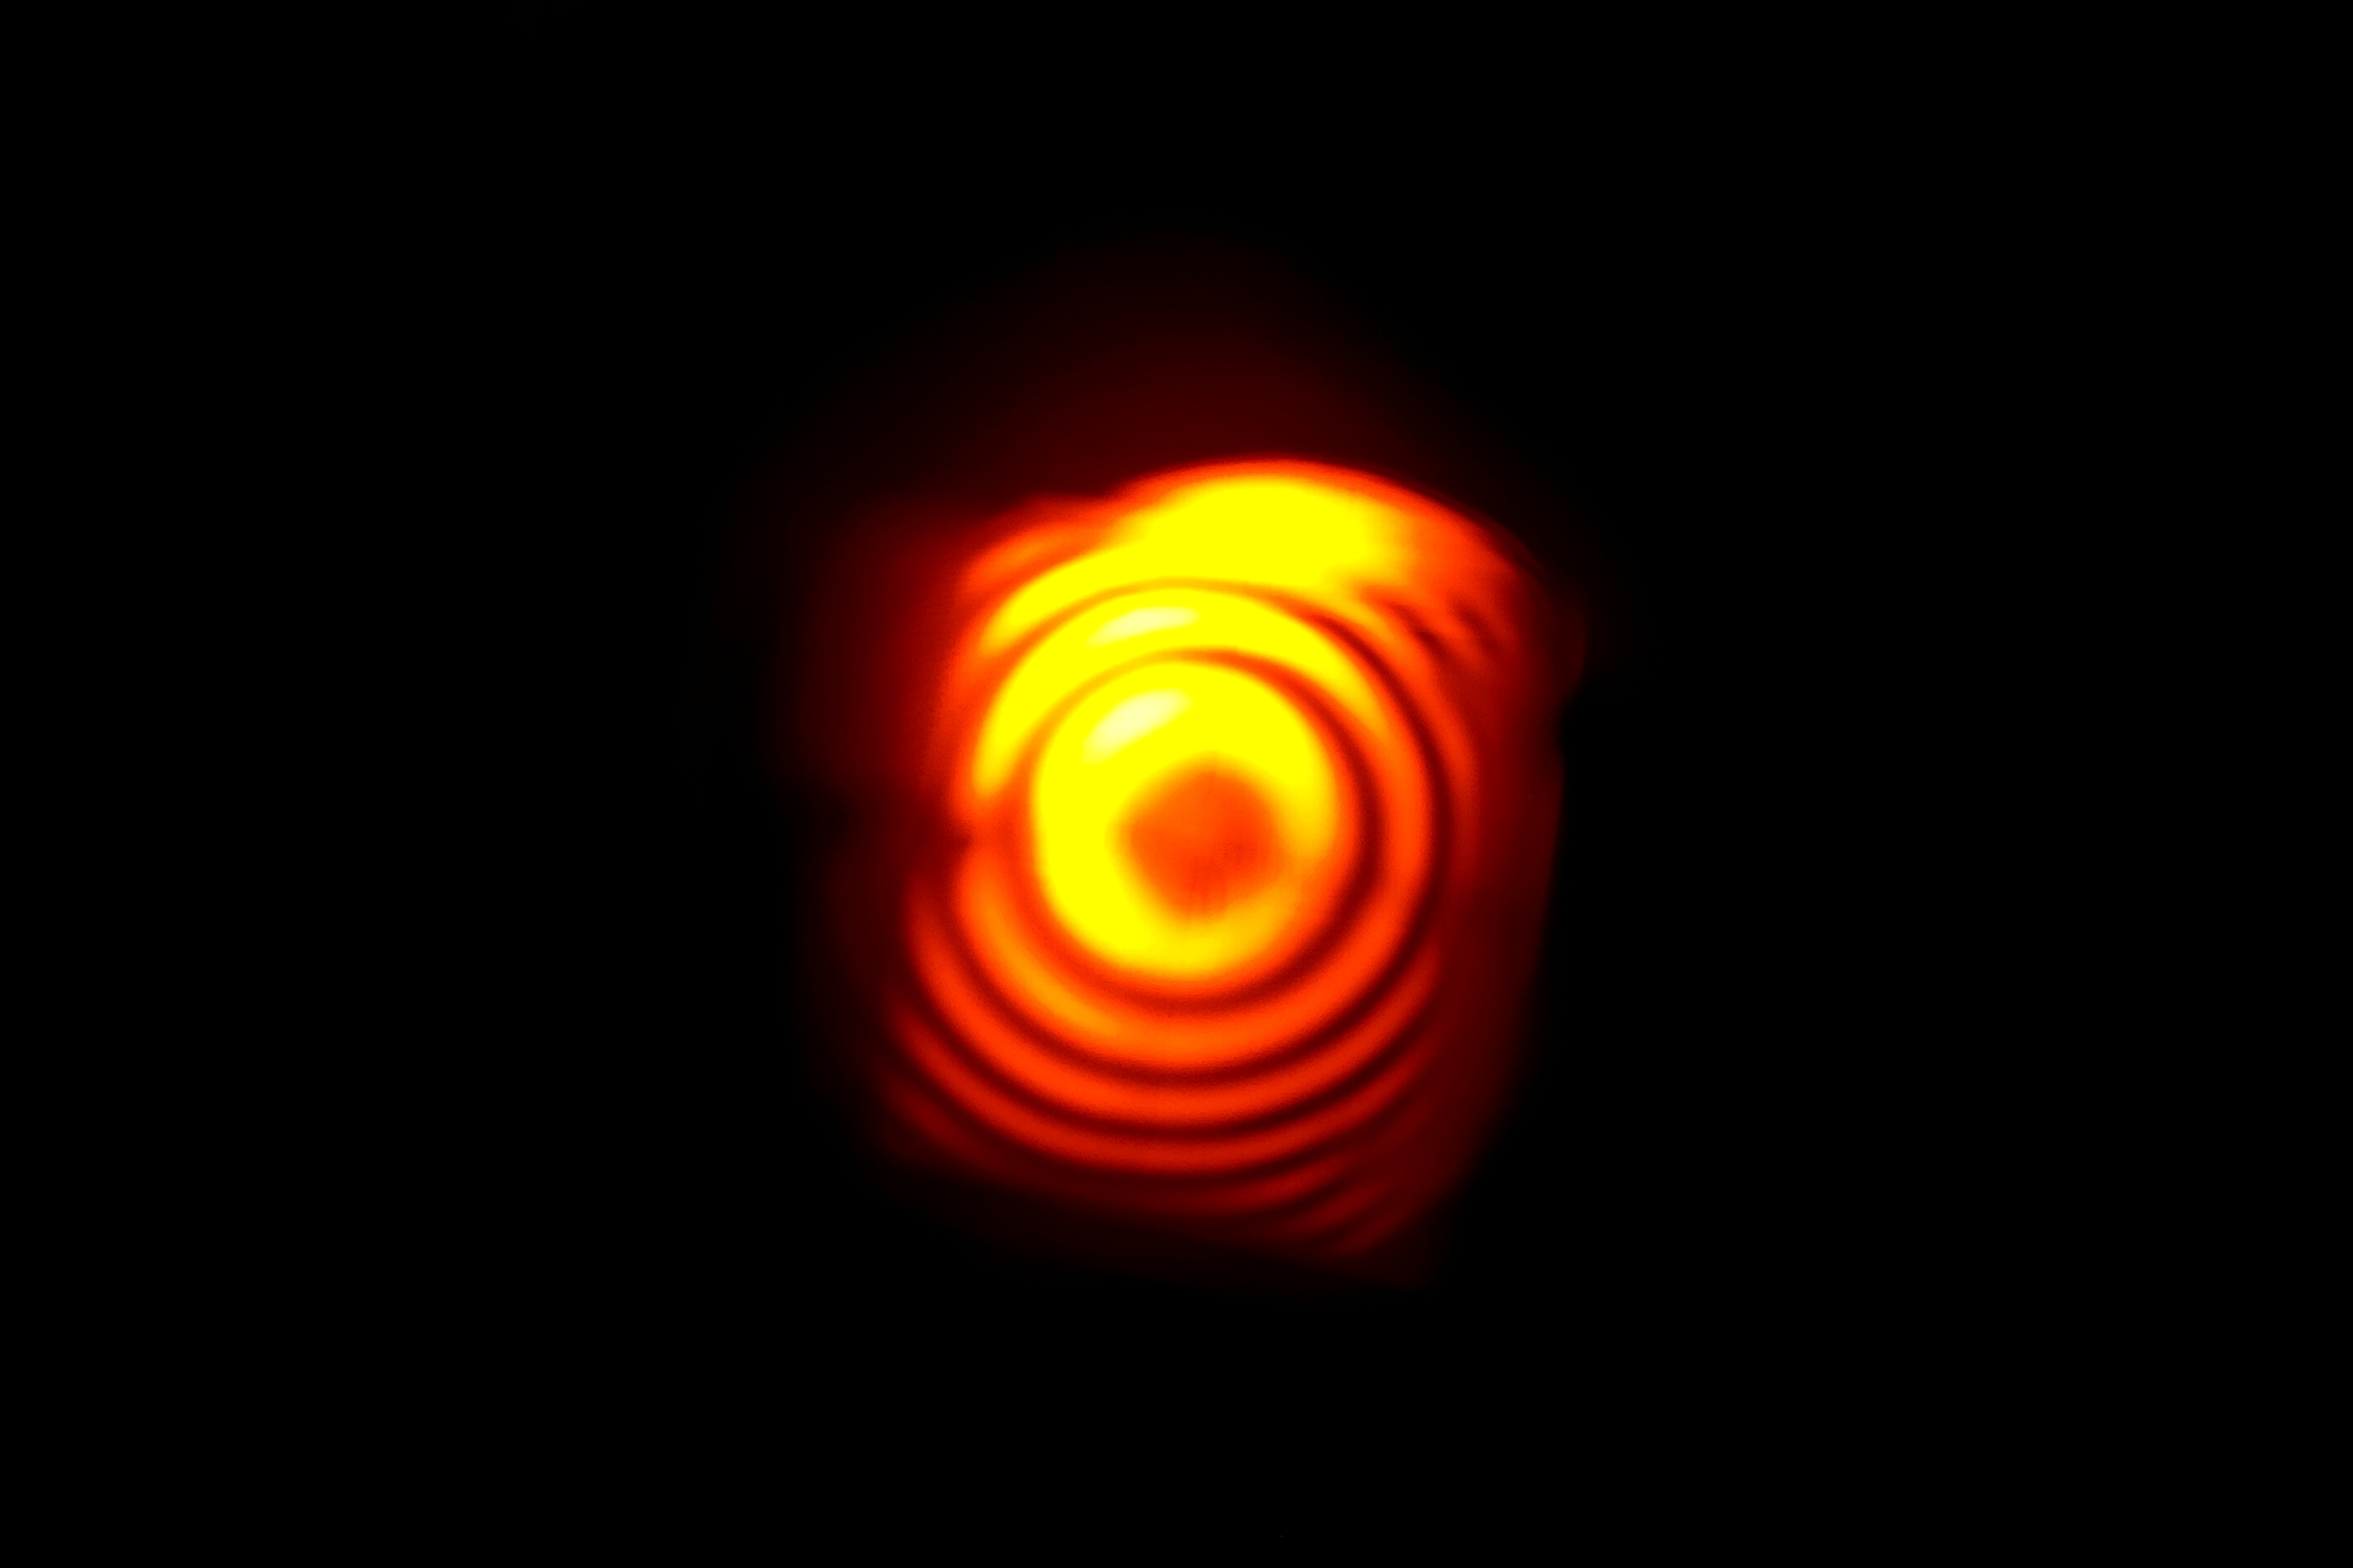
\includegraphics[width=0.8\linewidth]{./pic/eqicl.jpg}
    \caption{等倾干涉}
    \end{minipage}
    \begin{minipage}[t]{0.5\linewidth}
    \centering
    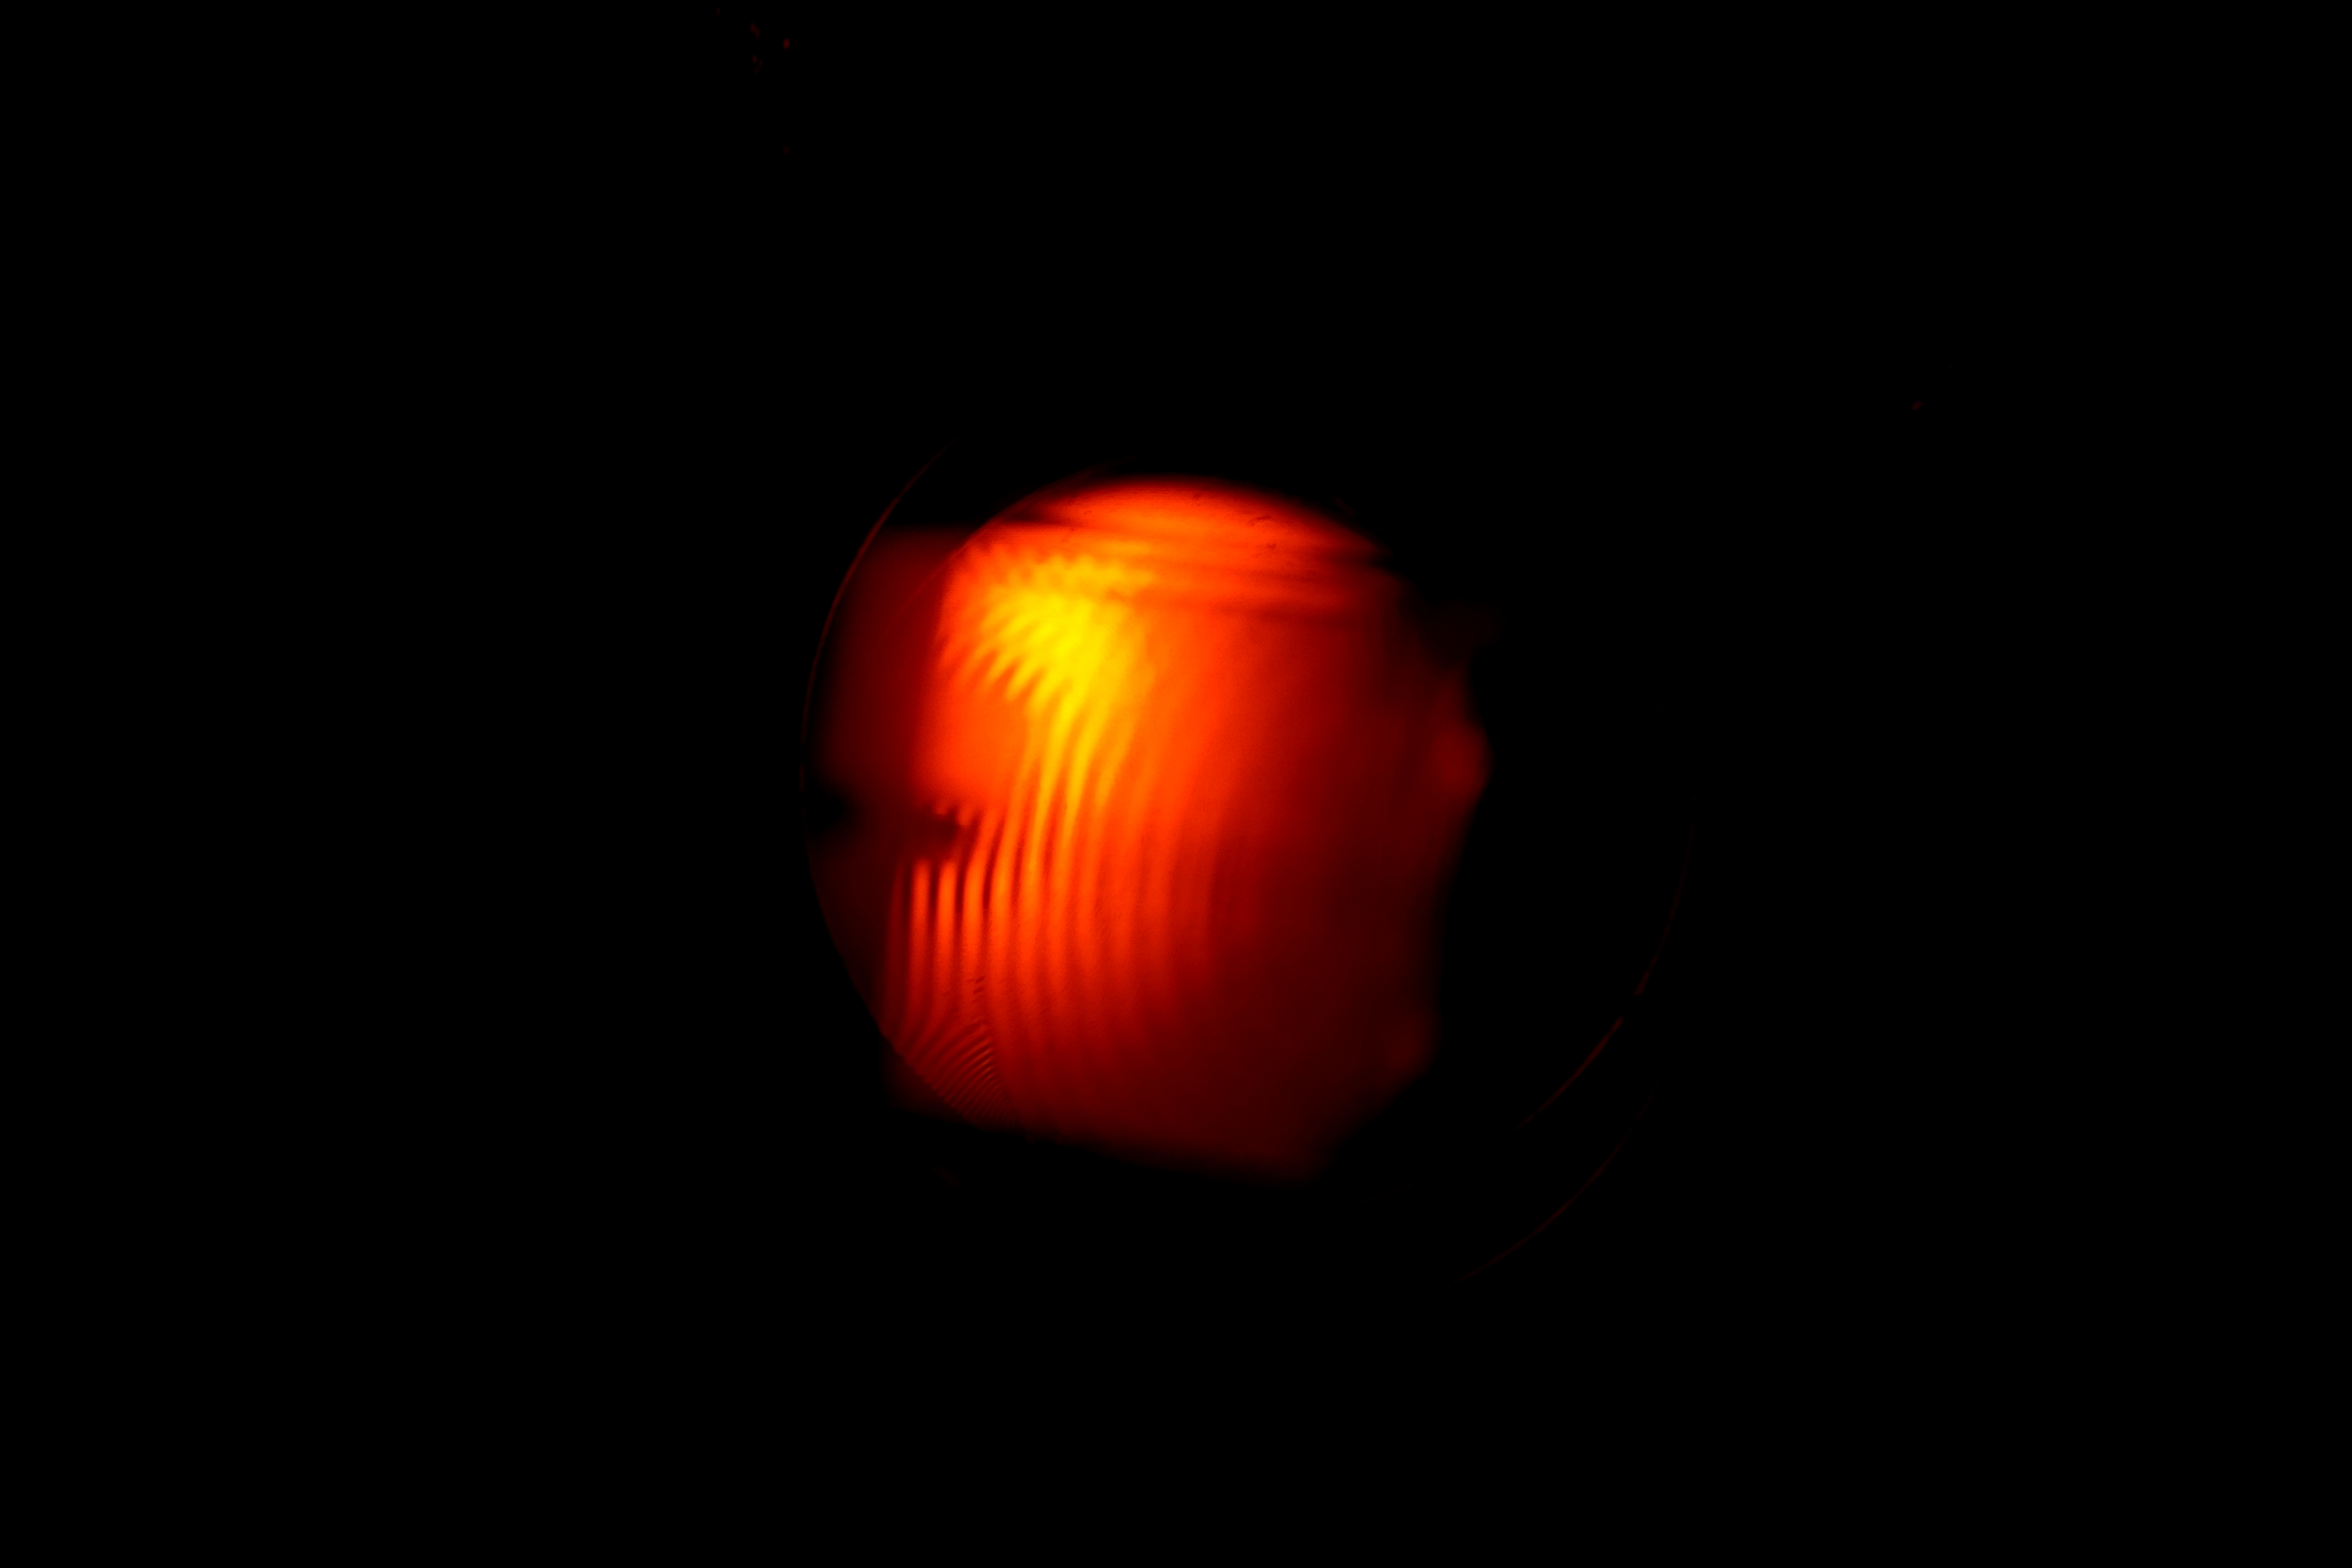
\includegraphics[width=0.8\linewidth]{./pic/eqthk.jpg}
    \caption{等厚干涉}
    \end{minipage}
\end{figure}

\begin{tikzpicture}[remember picture,overlay]
    \node[anchor=south east,inner sep=100pt] at (current page.south east) {
        \renewcommand{\arraystretch}{1.5} % 表格行高倍数
        \setlength{\tabcolsep}{18pt}    
    \begin{tabular}{|c|c|}
        \hline
        \LARGE  教师 & \LARGE  姓名 \\
        \hline
        \LARGE \kaishu 签字 &  \\
        \hline
        \end{tabular}
    };
\end{tikzpicture}

\newpage

\section{数据处理}
\subsection{利用逐差法计算氦-氖激光波长}

由光学知识可推导得变化了 k 个环时,已知测微器变化距离 d,可根据此式求出波长:

$$ k\lambda = 2 \times \frac{d}{20} = \frac{d}{10} $$

利用逐差法计算$\overline{\lambda}$

$$\overline{\lambda}=\frac{\sum\limits_{i=1}^{3} d_{i+3}-d_i }{10\times3^2\times50} = 642.2 \ nm$$
\subsection{作出条纹变化数$\Delta n$相对于气压变化$\Delta p$的曲线,用图解法计算斜率,求出空气的折射率。(想想还有什么其他合适的方法,也可以采用,不一定非要用图解法)}

取$ \Delta n = \overline{N} $并使用最小二乘法:

$$ \widehat{k} = \frac{\sum\limits_{i=0}^{5}\Delta n_i \Delta p_i - 6\overline{\Delta n} \ \overline{\Delta p}}{\sum\limits_{i=0}^{5}\Delta  p_i^2-6\overline{\Delta p}^2} = 0.08891428 $$

$$ \widehat{b} = \Delta n - \widehat{k} \ \overline{\Delta p} = -0.01422857 $$

绘出图像

\begin{figure}[h]
    \centering
    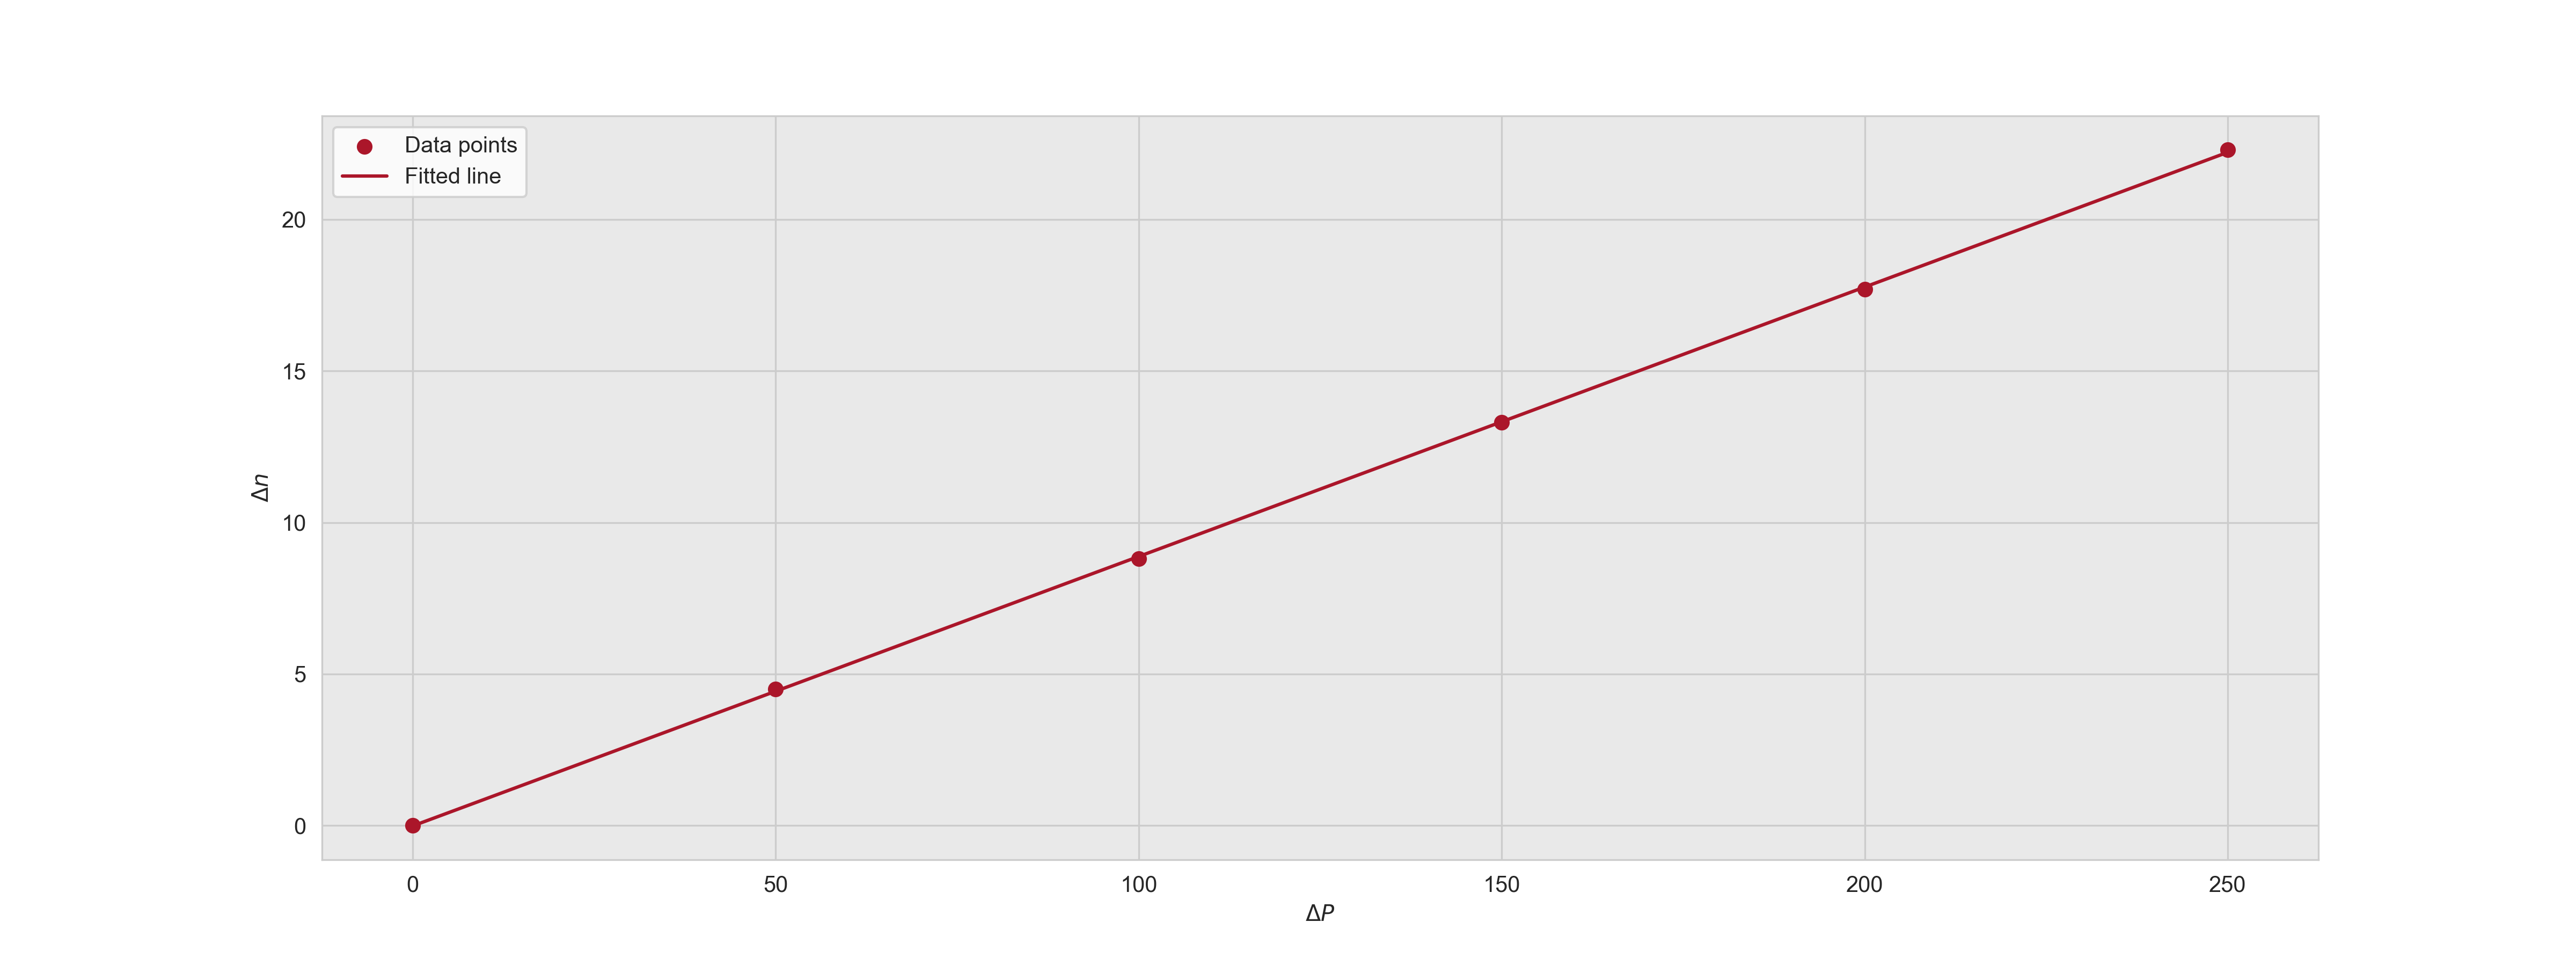
\includegraphics[width=\textwidth]{./pic/plot.png}
    \caption{拟合直线}
    \label{fig: data}
\end{figure}

空气折射率:

$$ n = 1 + \frac{\overline{\lambda} P_{amb}}{2l}\cdot \frac{\Delta n}{\Delta P} = 1 + \frac{\widehat{k} \ \overline{\lambda} P_{amb}}{2l} = 1.0002712 $$

\subsection{记录等倾和等厚现象、特点并分析。}

等倾条纹的特点是同心圆环,且中间较疏,越向外越密。这是因为同一特定光程差的干涉发生在某距成像中心的特定距离,这自然是圆环。 

等厚条纹的特点是平行明暗条纹。定镜、动镜像夹角极小时,可视作其间存在一线性空气薄层,可以发生等厚干涉。                                                               

经过仔细调节,可认为成功将动镜反射中心的像成在定镜反射中心处。调节观察位置可得到比较标准的直平行等厚条纹。 

\section{讨论题}

\subsection{归纳非定域干涉和定域干涉的特点。}

图片见数据记录页。

对于相干性较差的光源,在调整光路得到干涉条纹的过程中,只能在较小的调节范围(数厘米)内看到清晰的干涉条纹,即定域干涉。需要缓慢地调节出对应的图样。 

对于相干性较好的光源,在调整光路得到干涉条纹的过程中,可以在较大的调节范围(数米)内看到清晰的干涉条纹,即非定域干涉。往往不用特意调节就可以产生干涉条纹。 

\subsection{迈克尔孙干涉仪所产生的干涉条纹疏密程度是由什么因素决定的?变化规律怎样?}

干涉条纹的变化根源在于光程差的改变。当某一点的干涉条纹变得更密时,这是因为该点附近的光程差变化速度加快了。本实验中的压力气室实验正是基于这一原理,增加气压会导致折射率增大,从而使条纹更密集。此外,调整动镜和定镜的角度和高度也会引起条纹密度的变化。这是因为光路的整体变化导致对应点的光程差发生了改变,条纹疏密也大概率会发生变化。
\subsection{说明仪器要设计补偿片的原因。}

\begin{wrapfigure}{r}{0.4\textwidth} % 纵向8行,图片靠右,宽度12.5em
    \begin{center}
        \vspace{-1cm}
        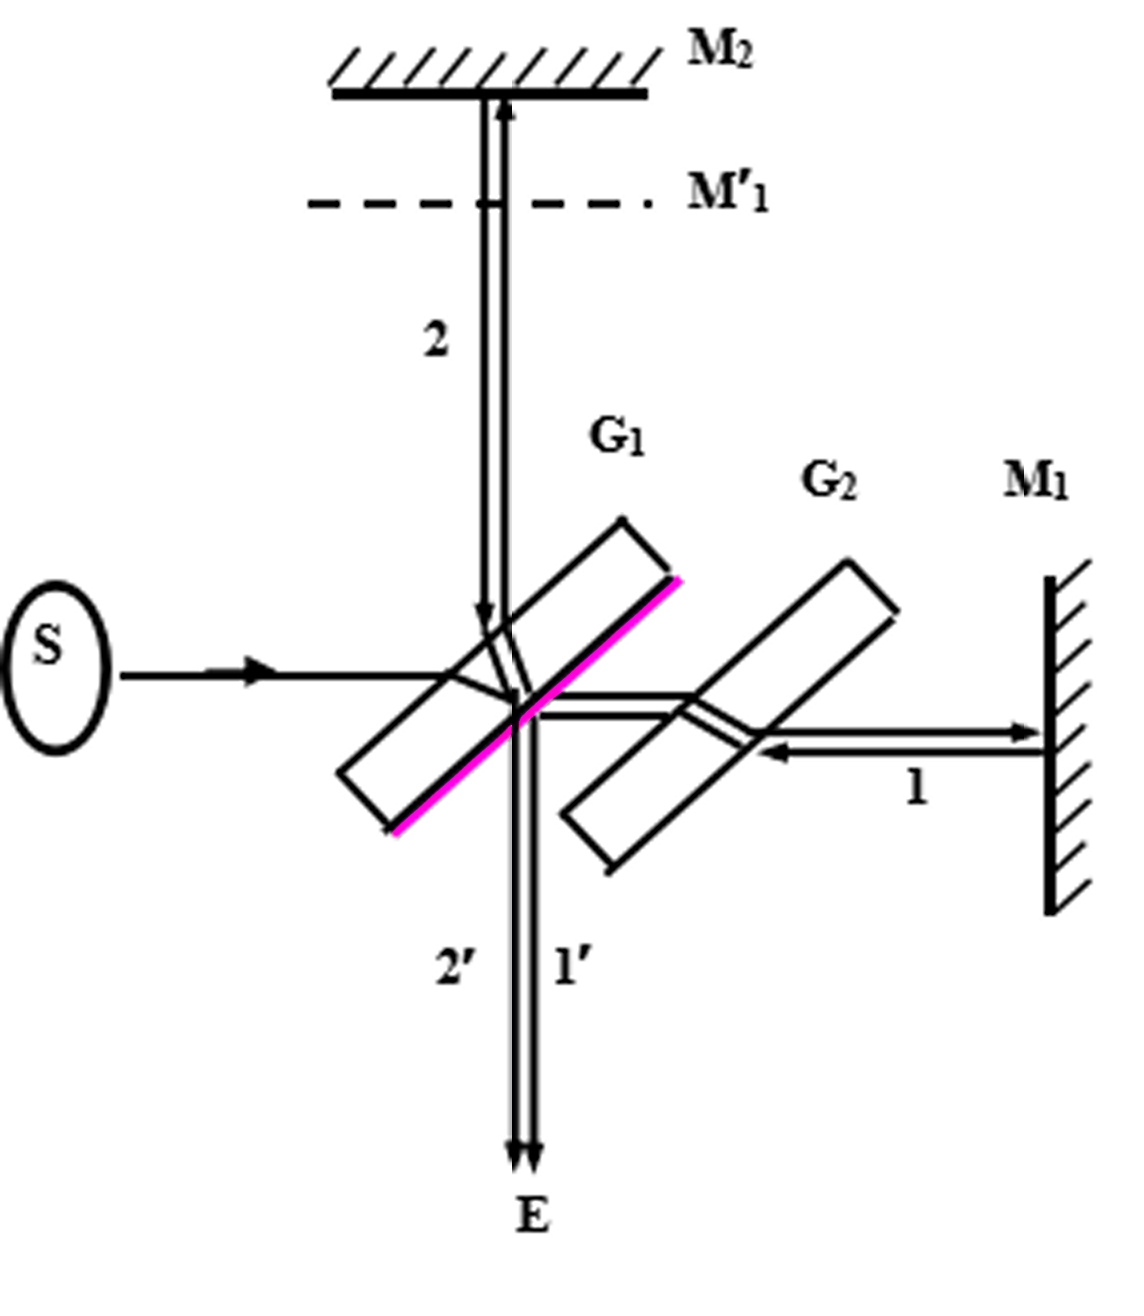
\includegraphics[width=0.25\textwidth]{./pic/rt.png}
        \label{fig:route}
    \end{center}
    \caption{光路}
\end{wrapfigure}
在半透半反镜和动镜之间放置的补偿板与半透半反镜的厚度相等,并且方向平行。该补偿板的目的是确保透射光和反射光的光程相等。如果没有补偿板,在不考虑多次反射透射的情况下,被半透半反镜反射出的光会经过该半透半反镜片两次,而被半透半反镜透射的光则不会再次穿过该半透半反镜。这将导致两束光的光程相差两倍半透半反镜的光程。为了消除这种误差,需要设计了一个补偿片,如图示。

\end{document}